\begin{abstract}
	Les algorithmes génétiques appartiennent à la famille des algorithmes évolutionnaires. Ils permettent d'obtenir une solution approchée ou exacte à un problème d'optimisation. Au nombre de ces algorithmes génétiques figurent une catégorie connue sous le nom d'algorithmes génétiques parallèles. En combinant ces différents algorithmes génétiques parallèles \cite{cant2}, l'on obtient alors des algorithmes génétiques parallèles et hiérarchiques encore plus efficaces. 
\end{abstract}

\section*{Introduction}
	\addcontentsline{toc}{section}{Introduction}
	 Dans ce chapitre, nous présentons dans un premier temps les outils de test utilisés, puis le modèle utilisé dans notre étude afin de représenter les instances de PSP et ensuite les aspects généraux ou communs à nos deux approches heuristiques basées sur les algorithmes génétiques. Dans un second temps, nous décrivons ces deux méthodes de recherche en nous appuyant sur les algorithmes implémentés.
	
	\section{Outils de test} 
		\subsection{Matériel}
		Pour l'implémentation de nos tests, nous avons travaillé sur un ordinateur présentant les caractéristiques suivantes :\\
		\begin{itemize}
			\item[•] Système d'exploitation: Linux Ubuntu 16.04 LTS; 
			\item[•] Processeur: Intel®  Core \up{\textsc{TM}} i7 CPU L 640 @ 2.13GHz x 4; 
			\item[•] Mémoire: 3,7 Gio;
			\item[•] Type du système d'exploitation: 64 bits.
		\end{itemize}
		
		\subsection{Langage de programmation}
		Le langage de programmation utilisé afin d'implémenter nos deux approches est le langage \emph{Python} dans sa version Python 3.5. \emph{Python} est un langage de programmation interprété et orienté objet. Il est placé sous une licence libre et fonctionne sur la plupart des plate-formes informatiques \cite{wikipedia_python}.
	
	\section{Modèle et formulation utilisés}
	Dans le but de modéliser et de formuler les instances de PSP, nous nous sommes servis de la première formulation en programmation en nombres entiers (MIP1). Nous rappelons ici ce modèle. 
	
	\begin{eqnarray}
		min \sum_{i,j,t} q^{i,j}\chi_{t}^{i,j} + \sum_{i,t} h^{i} s_{t}^{i} \\
		s_{0}^{i} = 0, \forall i \\
		x_{t}^{i} + s_{t-1}^{i} = d_{t}^{i} + s_{t}^{i}, \forall i,t \\
		x_{t}^{i} \leq y_{t}^{i}, \forall i,t \\
		\sum_{i} y_{t}^{i} = 1 , \forall t \\
		\chi_{t}^{i,j} = y_{t-1}^{i} + y_{t}^{j} - 1, \forall i,j,t \\
		x,y,\chi \in \{0,1\}, s \in \mathbb{N}, i \in \{0..NI\}, t \in \{1..NT\}
	\end{eqnarray}
		
		avec les variables de décisions suivantes: \\
		\begin{itemize}
			\item[-] $x_{t}^{i}$ : variable binaire de production qui vaut 1 si l’article $i$ est produit à la période $t$ et 0 sinon ;
			\item[-] $y_{t}^{i}$ : variable binaire de setup qui vaut 1 si la machine est préparée pour la production de l’article $i$ et 0 sinon ;
			\item[-] $s_{t}^{i}$ : variable entière de stockage qui contient le nombre d’articles $i$ stockés à la période $t$ ; 
			\item[-] $\chi_{t}^{i,j}$ : variable binaire de transition qui vaut 1 si à la période $t$, on est passé de la production de l’article $i$ à l’article $j$ et 0 sinon.
		\end{itemize}
	
	\section{Aspects généraux aux deux méthodes de recherche proposées}
	\subsection{Représentation génétique}
	Différentes représentations peuvent être utilisées avec les techniques évolutionnaires telles que les algorithmes génétiques. La représentation la plus simple pour les algorithmes génétiques est celle utilisée par John Holland: une chaîne de bits. Une chaîne de bits est connue comme un chromosome, et chaque bit est un gène. En début d'étude, nous avons donc commencé par représenter un chromosome en chaîne de bits. \\
	\textsl{\textbf{Exemple}}:\\
	\hspace*{.5cm} En suivant l'exemple d'une instance de PSP en page \pageref{sec:problem_description}, nous pouvons représenter un chromosome conformément à la figure \ref{fig:init_gene_repr}.
	
	\begin{figure}[h]
		\begin{center}
			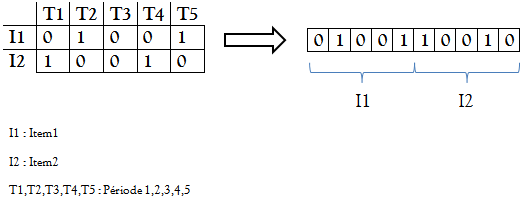
\includegraphics[scale=.5]{images/init_gene_repr.png}
			\caption{Représentation génétique initiale}
			\label{fig:init_gene_repr}
		\end{center}
	\end{figure}
	
	Autrement dit:
	\begin{center}
		$ch_{T} = \{(x_{1,1}),..., (x_{1,t+1}),..., ( x_{1,T}), (x_{i+1,1}),...,(x_{i+1, t+1}),..., (x_{i+1,T}),..., (x_{I,T})\}$ \\
	\end{center}
	\hspace*{.5cm} où $ch_{T}$ est un chromosome dont l'horizon de planification est de $T$ périodes et $x_{it}$ est la variable booléenne qui indique la production ou non d'un article \emph{i} en période \emph{t}.  \\
	\\
	\hspace*{.5cm} Dans cette représentation, un chromosome est une chaîne de bits (0 et 1) qui indique la production ou non d'un article \emph{i} et de longueur \emph{nItems * nTimes} (où \emph{nItems} est le nombre d'articles et \emph{nTimes} est le nombre de périodes). Ainsi, l'article 1 est produit dans les périodes 2 et 5; et l'article 2 est produit dans les périodes 1 et 4. Le chromosome représenté ci-dessus est ainsi un plan de production qui satisfait aux contraintes du système de production spécifiques à cette instance du problème. Toutefois, au cours de notre étude, une seconde représentation nous est apparue plus facilement manipulable. Cette représentation génétique est présentée à la figure \ref{fig:adopt_gene_repr} et étudiée par Mirshekarian et al. \cite{suer}.
	
	\begin{figure}[!h]
		\begin{center}
			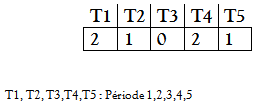
\includegraphics[scale=.5]{images/adopt_gene_repr.png}
			\caption{Représentation génétique adoptée}
			\label{fig:adopt_gene_repr}
		\end{center}
	\end{figure}
	
	Dans cette représentation, un chromosome est une suite d'entiers correspondant aux articles produits et de longueur \emph{nTimes}. La longueur réduite de ce chromosome réduit dans le même temps la durée du parcours du chromosome lors des implémentations.
	\subsection{Initialisation}
	Le processus d'initialisation consiste à construire la population initiale; c'est à dire celle à partir de laquelle se feront les opérations de sélection, croisement ou encore mutation afin de la faire évoluer sur des générations. L'initialisation au niveau des algorithmes génétiques se fait de manière aléatoire dans l'optique de trouver des individus suffisamment différents capables de constituer une population diverse dans le but de largement couvrir l'espace de recherche. \\
	\hspace*{.5cm} Une autre approche consiste à créer les individus devant composer la population initiale en se servant de stratégies de recherche informées munies de fonctions d'évaluation menant à des bonnes solutions. Notre approche a été donc d'utiliser une stratégie de recherche en l’occurrence le "Hill Climbing" dotée d'une fonction d'évaluation afin de déterminer lequel des fils à considérer.\\
	\hspace*{.5cm} \textbf{\textsl{Principe:}}\\
	Le principe d'initialisation de la population est le suivant : remplir un chromosome en commençant par le dernier gène et en finissant par le premier. Cela permet de s'assurer de la faisabilité des solutions que nous trouvons au bout du processus. Ainsi, pour chaque gène visité, nous disposons de la liste des allèles qui peuvent prétendre occuper ce dernier, nous pouvons alors choisir l'allèle qui minimise le "fitness" du chromosome entrain d'être constitué.\\
	\hspace*{.5cm} \textbf{\textsl{Algorithme:}}\\	
	L'algorithme \ref{alg:generation_pop_init} détaille le processus de génération de la population initiale: \\
	
	\begin{algorithm}[H]
		\caption{Processus de génération de la population initiale}
		\label{alg:generation_pop_init}
 		\KwData{instance de PSP à traiter, taille de la population}
 		\BlankLine
 		\KwResult{Population initiale constituée}
		\BlankLine 		
		$queue \gets []$
		\BlankLine
		$noeud \gets nouveauNoeud()$ \\
		\BlankLine
 		\While{taille(populationInitiale) est inférieure à taillePopulation}{
 			\BlankLine
 			\eIf{noeud.chromosome est prêt}{
 				\BlankLine
 			 	populationInitiale.ajouter(noeud.chromosome)
 			 	\BlankLine
 			 }
 			 {
 			 	\BlankLine
 			 	$noeudFils \gets noeud.obtenirSuccesseurs()$ \\
 			 	\BlankLine
 			 	noeudFils.trier(decroissant) \\
 			 	\BlankLine
 			 	queue.ajouter(noeudFils)
 			 	\BlankLine
 			 	\If {queue est vide}
 			 	{
 			 		\BlankLine
 			 		\Return populationInitiale
 			 		\BlankLine
 			 	}
 			 	\BlankLine
 			 	$noeud \gets  queue.dernier()$
 			 }	
	}
	\Return populationInitiale
	\end{algorithm}	
	
	L'algorithme \ref{alg:generation_successeurs} décrit la génération des successeurs d'un noeud donné.
	\begin{algorithm}
		\caption{Processus de génération des successeurs d'un noeud}
		\label{alg:generation_successeurs}
 		\KwData{noeud}
 		\BlankLine
 		\KwResult{liste des successeurs constituée}
		\BlankLine 		
		$successeurs \gets []$
		\BlankLine
		\For{ article $\gets$ nombreArticles $\KwTo$ 1}
		{
			\BlankLine
			\If{article.dernierDeadline $>=$ noeud.positionActuelle}
			{
				\BlankLine
				noeudFils = copie(noeud)
				\BlankLine
				noeudFils.positionActuelle -= 1
				\BlankLine
				successeurs.ajouter(noeudFils)
				\BlankLine
			}
		}
	\Return successeurs
	\end{algorithm}	
	
	\hspace*{.5cm} \textbf{\textsl{Description de l'algorithme:}}\\	
	L
	
	\hspace*{.5cm} La figure \ref{fig:hill_climbing_fig} présente un schéma illustratif de l'application de l'algorithme du Hill climbing à l'instance de PSP détaillé en page \pageref{sec:problem_description}. A travers cette figure et en appliquant notre algorithme basé sur le hill climbing, le nœud "\emph{fils}" de gauche sera choisi sur le nœud "\emph{fils}"  de droite car il présente une valeur de coût inférieure.
	
	\begin{figure}[!h]
			\begin{center}
				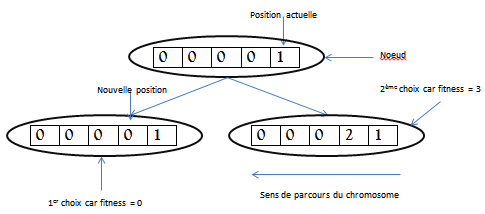
\includegraphics[scale=.7]{images/hill_climbing_fig.png}
				\caption{Schéma illustratif de l'application de l'algorithme du Hill climbing à une instance de PSP}
				\label{fig:hill_climbing_fig}
			\end{center}
	\end{figure}
	
	\subsection{Opérateurs génétiques}
		\subsubsection{Sélection}
		
		\hspace*{.5cm} Dans notre étude, nous choisissons de nous intéresser à la plus connue et commune d'entre les méthodes de sélection et qui offre en général des résultats intéressants sur ce genre de problèmes: le \emph{"Roulette Wheel"}. Rappelons que dans la sélection par "\emph{roulette wheel}", les individus se voient attribués une probabilité d'être sélectionnés, proportionnelle à leur fonction d'évaluation dans le but de produire des "\emph{fils}". Ces "\emph{fils}" sont ainsi de nouvelles solutions au problème et forment une nouvelle population.		
		
		\subsubsection{Croisement}
		
		Une fois les individus sélectionnés, intervient le croisement. Le croisement en un point a été choisi afin de reproduire ces individus. La figure \ref{fig:used_cross_over} présente une illustration du croisement appliqué à l'instance de PSP introduite à la page \pageref{sec:problem_description}.
		\begin{figure}[!h]
			\begin{center}
				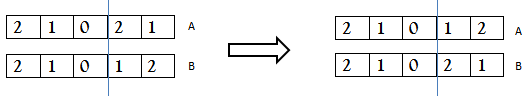
\includegraphics[scale=.5]{images/cross_over_fig.png}
				\caption{Illustration du croisement utilisé}
				\label{fig:used_cross_over}
			\end{center}
		\end{figure}
		
		Le croisement se fait ici après la troisième période. Le croisement peut engendrer des individus qui, contrairement à la figure \ref{fig:used_cross_over}, ne respectent pas les contraintes de système en terme de \emph{shortage} ou de \emph{backlogging}. Il faut alors rendre ces individus à nouveau faisables avant de procéder à une quelconque mutation. L'algorithme \ref{alg:cross_over} présente le croisement implémenté dans le cadre de cette étude. Notons que notre algorithme a une complexité linéaire en $O(n)$ avec $n$, le nombre de périodes du problème à résoudre.\\
		
		\begin{algorithm}[H]
 		\caption{Algorithme de croisement utilisé}
 		\label{alg:cross_over}
 		\KwData{parent1, parent2, seuil\_probabilite}
 		\KwResult{child1 et child2}
 		\BlankLine
 		child1 $\gets$ $nouveau\ chromosome()$ \\
 		child2 $\gets$ $nouveau\ chromosome()$ \\
 		$probabilite \gets random(1,99)$ \\
 		\BlankLine
 		\If{probabilite $\leq$ seuil\_probabilite}
 		{
 			$nbGenes \gets NombreDeGenes(parent1)$\\
 			$indice\_gene \gets random(1, nbGenes)$\\
 			//$ Le \ nombre \ de \ genes \ du \ parent1 \ est \ le \ meme \ que \ celui \ du \ parent2 $\\
 			\For{ i $\gets$ 0 \KwTo nbGenes}
 			{
 				$gene1 \gets obtenirGene(parent1, i)$ \\
 				$gene2 \gets obtenirGene(parent2, i)$ \\
 				\eIf{i $\leq$ indice\_gene}
 				{
 					$child1.ajouterGene(gene)$ \\
 					$child2.ajouterGene(gene)$ \\
 				}
 				{
 					$child2.ajouterGene(gene)$ \\
 					$child1.ajouterGene(gene)$ \\
 				}
 			}
 		}
 		\Return{child1, child2}
		\end{algorithm}
		  
	\subsubsection{Mutation}
	Après la sélection et le croisement, une nouvelle population d'individus est prête. Certains ont été copiés directement et d'autres se sont reproduits par croisement. Dans le but de s'assurer que les individus ne sont pas exactement les mêmes, une mutation est appliquée à chacun des individus "\emph{fils}". Un visuel de la mutation appliquée à l'instance de PSP explicitée en section \ref{sec:problem_description} est présenté à la figure \ref{fig:used_mutation}.\\
	
	\hspace*{.5cm} \textbf{\textsl{Principe}}\\
	\hspace*{.5cm} L'objectif de notre algorithme de mutation est de parvenir à altérer la valeur d'un gène. Pour ce faire et dans le souci de conserver le chromosome comme étant une solution du problème, nous avons décidé de permuter les valeurs de gènes choisis de façon aléatoire. Ainsi, dans un premier temps, nous choisissons de façon aléatoire un gène à muter. Une fois que cela est fait, nous déterminons toujours aléatoirement une autre valeur d'article pour ce gène ou période. Cette nouvelle valeur nous permet, en partant de la période du premier gène (aléatoirement choisi) pour le premier gène du chromosome, de déterminer le premier gène ayant cette valeur et dont la date limite de demande est supérieure à notre premier gène aléatoirement choisi.
	
	\hspace*{.5cm} \textbf{\textsl{Algorithme}}\\
	\hspace*{.5cm} L'algorithme \ref{alg:mutation} détaille le processus utilisé afin de faire muter un chromosome. 
	
	\begin{figure}[!h]
		\begin{center}
			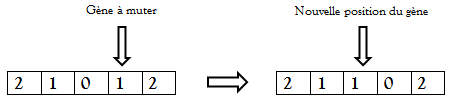
\includegraphics[scale=.5]{images/mutation_fig.png}
			\caption{Illustration de la méthode de mutation}
			\label{fig:used_mutation}
		\end{center}
	\end{figure}
	
	\begin{algorithm}[H]
 		\caption{Algorithme de mutation utilisé}
 		\label{alg:mutation}
 		\KwData{chromosome, seuil\_probabilite}
 		\KwResult{chromosome}
 		\BlankLine
 		$probabilite \gets random(1,99)$ \\
 		\BlankLine
 		\If{probabilite $\leq$ seuil\_probabilite}
 		{
 			\BlankLine
 			$nbGenes \gets NombreDeGenes(chromosome)$\\
 			\BlankLine
 			$indice\_gene \gets random(1, nbGenes)$\\
 			\BlankLine
 			$gene1 \gets obtenirGene(chromosome, indice\_gene)$ \\
 			\BlankLine
 			//$ Le \ nombre \ de \ genes \ du \ parent1 \ est \ le \ meme \ que \ celui \ du \ parent2 $\\
 			\BlankLine
 			\For{ i $\gets$ indice\_gene \KwTo 0}
 			{
 				\BlankLine
 				$gene2 \gets obtenirGene(chromosome, i)$\\
 				\BlankLine
 				\If{deadline(gene2) $>=$ indice\_gene}
 				{
 					\BlankLine
 					$deplacer(gene1, gene2, chromosome)$ \\
 					\BlankLine
 					$arret$
 					\BlankLine
 				}
 			}
 		}
 		\Return{chromosome}
		\end{algorithm}
		
	\vspace*{.3cm}		
	\hspace*{.5cm} \textbf{\textsl{Description de l'algorithme}} \\
	\hspace*{.5cm} L'algorithme de mutation utilisé dans le cadre de notre travail prend en entrée un objet de type chromosome avec un seuil de probabilité de mutation et retourne ce même objet \emph{chromosome} modifié. Au cours du processus, la primitive \emph{random()} retourne une probabilité de mutation. Dans le cas où cette probabilité est supérieure au seuil de probabilité défini en entrée, la mutation survient. Nous récupérons alors le nombre de gènes du chromosome pour le problème à résoudre à l'aide de la primitive \emph{NombreDeGenes()}. Notons que ce nombre de gènes est égal au nombre de périodes défini dans le problème. La primitive \emph{random()} nous permet de déterminer de tous les gènes, lequel muter. Ce gène est ainsi récupérer à l'aide de \emph{obtenirGene()}. En fin de processus, une fois les deux gènes à permuter connus, la primitive \emph{déplacer()} nous permet d'effectuer la permutation.
	
	
	
	\subsection{Évaluation}
	L'évaluation dans notre étude se réfère à la fonction objectif. Il s'agit de minimiser les coûts d'exploitation et de production. Deux types de coût sont à prendre en compte:
	\begin{itemize}
		\item[•] Les coûts de preparation ou \emph{setup} sont des coûts induits au moment d'un changement dans la configuration d'une ressource d'un type d'article à un autre. Il s'agit de perte potentielle de production durant la période de préparation, de force de travail additionnelle ou encore de ressources additionnelles brutes consommées durant la préparation.
		\item[•] Les coûts de stockage qui sont induits lors du conditionnement et d’entreposage.
	\end{itemize}
	L'algorithme \ref{alg:evaluation} explicite le processus suivi afin d'évaluer un chromosome. Notre algorithme possède une complexité linéaire en O(n). En effet, la fonction d'évaluation est une fonction qui détermine le fitness de nouveaux individus ou chromosomes. Ainsi, disposer une complexité linéaire sur cet algorithme est important afin de garder nos méthodes de recherche compétitives sur de grandes instances.
	
	\begin{algorithm}[H]
 		\caption{Algorithme utilisé dans le processus d'évaluation d'un chromosome}
 		\label{alg:evaluation}
 		\KwData{chromosome, cout\_stockage, cout\_transition}
 		\KwResult{eval}
 		\BlankLine
 		$eval \gets 0$\\
 		$// On\ calcule\ le\ cout\ de\ stockage\ de\ chaque\ production$ \\
 		\For{gene in chromosome}{
 			\If{gene.value != 0}{		
 				$date\_limite \gets getDateLimite(gene)$ \\
 				$temp \gets (date\_limite\ -\ gene.periode) * cout\_stockage(gene.value)$ \\
 				$evaluation \gets evaluation\ +\ temp$ \\
 			}
 		}
 		$// On\ calcule\ le\ cout\ de\ transition\ de\ entre\ deux\ productions$ \\
 		\For{gene in chromosome}{
 			\If{gene.valeur != 0}{		
 				$next\_gene \gets obtenirProchainGene(chromosome)$ \\
 				\If{transition(gene, prochain\_gene) est vrai}{
 					$temp \gets cout\_transition(gene, prochain\_gene)$\\
 					$evaluation \gets evaluation\ +\ temp$
 				}
 			}
 		}
 		\Return{evaluation}
	\end{algorithm}
	
	\subsection{Terminaison}
	Deux moyens sont utilisés par lesquels les algorithmes génétiques se terminent. Habituellement, une limite est mise sur le nombre de générations après lesquelles le processus se termine. Avec certains problèmes, le processus de recherche se termine quand une solution particulière a été trouvée ou encore lorsque la plus haute valeur de "fitness" dans la population a atteint une valeur particulière. \\
	\hspace*{.5cm} Le critère de terminaison utilisé dans notre étude afin de terminer une recherche est le suivant : la recherche se termine lorsque l'algorithme converge sur un individu considéré comme une solution optimale. A cet optimal local, est appliqué une fonction de recherche locale afin de déterminer dans l'entourage immédiat de cet individu, un autre individu de meilleure qualité. Dans le cas, où un meilleur individu ne serait pas trouvé, la recherche s’arrête donc sur cet optimal local.
	
	\subsection{Fonction de la faisabilité}
	Le croisement et la mutation sont tous des opérateurs génétiques qui produisent en sortie des chromosomes. En fonction du gène muté dans le cas de la mutation ou du point de croisement dans le cas du croisement, ces chromosomes peuvent ne pas être faisables; c'est-à-dire qu'ils ne représentent pas des solutions au problème à résoudre. Il importe donc de les rendre à nouveau faisable. La fonction de faisabilité permet de rendre un chromosome ou individu à nouveau faisable. \\
	
	\hspace*{.5cm} \textbf{\textsl{Principe:}}\\	
	\hspace*{.5cm} Dans le but de rendre un chromosome faisable, nous  réduisons le surplus de production dans le cas d'un surplus et augmentons la quantité d'articles produits dans le cas d'un manque de production. Concrètement, il s'agit dans un premier temps de parcourir le chromosome à la recherche, pour chaque date limite de demandes, de surplus de production que nous avons supprimée. Dans un second temps, nous avons, pour chaque demande, vérifié si elle était satisfaite. Dans le cas où la demande n'était pas satisfaite alors, nous produisons un article correspondant à la demande. \\
	
	\hspace*{.5cm} \textbf{\textsl{Algorithme:}}\\	
	\hspace*{.5cm} L'algorithme \ref{alg:faisabilite} est celui utilisé dans l'objectif de rendre un chromosome faisable.
	\\
	\begin{algorithm}[H]
 		\caption{Algorithme utilisé comme fonction de faisabilité}
 		\label{alg:faisabilite}
 		\KwData{chromosome, deadlines}
 		\KwResult{eval}
 		\BlankLine
 		$//\ On\ commence\ par\ reduire\ le\ surplus\ de\ production$ \;
 		\For { $i \gets 1$ \KwTo Nombre\_Periodes}
 		{
 			article $\gets$ chromosome.obtenirArticle(i) \;
 			\If {estEnSurplus(article, deadline(i))}
 			{
 				supprimerProduction(article) \;
 			}
 		}
 		
 		$ //\ On\ compense\ le\ manque\ de\ production $ \;
 		
 		\For{ article in liste\_articles }
 		{
 			article\_deadlines $\gets$ deadlines(article) \;
 			\For{ deadline in article\_deadlines}
 			{
 				\If{nonProduit(dealine)}
 				{
 					produire(article)\;
 				}
 			}
 		}
 	
	\end{algorithm}
	
	\vspace*{.3cm}
	\hspace*{.5cm} \textbf{\textsl{Description de l'algorithme:}}\\	
	
	\section{Méthodes de recherche proposées}	
	
	Nous nous intéressons dans notre étude à appliquer les algorithmes génétiques parallèles et hiérarchiques "\emph{coarse-grained}" et "\emph{fine-grained}" et les algorithmes génétiques parallèles et hiérarchiques "\emph{coarse-grained}" et "\emph{master-slave}" présentés en page en section \ref{sec:algo_hierarchique}. Nous exposons les choix effectués dans le processus d'implémentation de ces algorithmes génétiques.
	
	\subsection{Algorithmes génétiques parallèles et hiérarchiques \emph{coarse-grained} et \emph{master-slave}}
		
	En implémentant les algorithmes génétiques parallèles et hiérarchiques \emph{coarse-grained} et \emph{master-slave}, nous avons effectué des choix en relation avec trois grands points importants. Il s'agit de la fréquence de migration, du nombre de migrants, de la topologie de connexion et de la méthode d'intégration des migrants.
	 
	\subsubsection{Fréquence de migration}
	
	\hspace*{.5cm} Dans l'implémentation des algorithmes génétiques parallèles et hiérarchiques \emph{coarse-grained} et \emph{master-slave}, nous avons donné à l'utilisateur la possibilité d'entrer l'intervalle de générations entre les migrations. Cependant, le comportement par défaut de l'algorithme est de migrer uniquement lorsque la population a convergé complètement.  
	
	\subsubsection{Choix et nombre de migrants}
	 Dans la suite de notre étude, nous avons choisi d'échanger les meilleurs individus. Nous rappelons la sélection des meilleurs individus peut aider à disséminer un matériel génétique qui a déjà été testé et qui serait donc intéressant au contraire de la sélection aléatoire des "migrants".
	 
	\subsubsection{Topologie de connexions}
	La topologie utilisée a été celle densément connectée présentée à la figure \ref{fig:topology_fig}. Dans cette topologie, tout nœud ou processus pris individuellement est le voisin logique de tous les autres nœuds de la topologie.
	
	\begin{figure}[!h]
		\begin{center}
			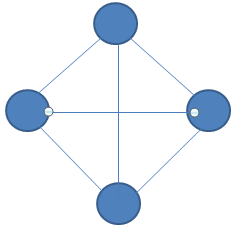
\includegraphics[scale=.3]{images/topology_fig.png}
			\caption{Topologie de connexions utilisée}
			\label{fig:topology_fig}
		\end{center}
	\end{figure}
	
	\subsubsection{Méthode d'intégration des migrants}
 	
 	Nous avons appliqué un remplacement compétitif à notre programme. Il s'est agi d'identifier les plus mauvais chromosomes en terme de fitness et de les remplacer par les nouveaux arrivants.
 	
	\subsection{Algorithmes génétiques parallèles et hiérarchiques \emph{coarse-grained} et \emph{fine-grained}}
	
	L'implémentation des algorithmes génétiques parallèles et hiérarchiques \emph{coarse-grained} et \emph{fine-grained} a suivi le même processus que celui des Algorithmes génétiques parallèles et hiérarchiques \emph{coarse-grained} et \emph{master-slave}. Les mêmes questionnements quant à la fréquence de migration, à la topologie de connexion, à la méthode d'intégration et au nombre de migrants sont revenus.
	
	\subsubsection{Fréquence de migration}
	
	\hspace*{.5cm} Dans la même idée que l'implémentation des algorithmes génétiques parallèles et hiérarchiques \emph{coarse-grained} et \emph{master-slave}, nous avons donné à l'utilisateur la possibilité d'entrer l'intervalle de générations entre les migrations. Cependant, le comportement par défaut de l'algorithme est de migrer uniquement lorsque la population a convergé complètement.  
	
	\subsubsection{Choix et nombre de migrants}
	 Afin de sélectionner les migrants nous avons choisi d'échanger les meilleurs individus. Nous rappelons la sélection des meilleurs individus peut aider à disséminer un matériel génétique qui a déjà été testé et qui serait donc intéressant au contraire de la sélection aléatoire des "migrants".
	
	\subsubsection{Méthode d'intégration des migrants}
 	
 	Nous avons appliqué un remplacement compétitif à notre programme. Il s'est agi d'identifier les plus mauvais chromosomes en terme de fitness et de les remplacer par les nouveaux arrivants.
	
	\subsubsection{Topologie de connexions}
	
	La figure \ref{fig:fine_grained_fig} présente la topologie (grille 2-Dimension) utilisée afin d'implémenter l'algorithme génétique parallèle de type \emph{"fine-grained"}.
	
	\begin{figure}[!h]
		\begin{center}
			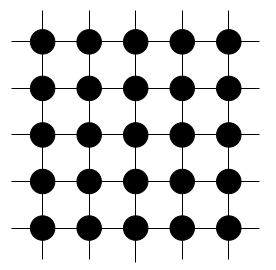
\includegraphics[scale=.3]{images/fine_grained_fig.png}
			\caption{Topologie utilisée en algorithme génétique parallèle de type "\emph{fine-grained}" \cite{cant2}}
			\label{fig:fine_grained_fig}
		\end{center}
	\end{figure} 
	
	\subsubsection{Algorithme hiérarchique entre \emph{fine-grained} et \emph{coarse-grained}}
	
	\subsection{Autres algorithmes implémentés}
	%Au cours de notre étude de l'art et en implémentant nos deux méthodes de résolution proposées que sont les algorithmes génétiques parallèles et hiérarchiques \emph{coarse-grained} et \emph{master-slave} et les algorithmes génétiques parallèles et hiérarchiques \emph{coarse-grained} et \emph{fine-grained}, nous avons pu découvrir différentes fonctions annexes aux algorithmes génétiques qui permettent d'en améliorer la qualité. Il s'agit des méthodes d'hybridation \cite{Goncalves} et de table de hashage \cite{povinelli}.
	
	\subsubsection{Hybridation}
	\hspace*{.5cm} Dans notre étude, Nous avons mis au point un algorithme de recherche locale qui est utilisé à chaque fois que l'algorithme génétique converge sur une solution optimale afin de parcourir l'espace de recherche immédiat à cette solution et ainsi améliorer cette solution optimale. L'algorithme \ref{alg:local_search} décrit le processus suivi afin de chercher de meilleures solutions à partir d'un chromosome fourni en paramètre. Cet algorithme une complexité polynomiale en $O(n^{2})$ 
	\\
	\begin{algorithm}[H]
		\label{alg:local_search}
 		\caption{Algorithme de recherche locale d'une meilleure solution}
 		\KwData{individu à améliorer}
 		\BlankLine
 		\For{chaque gène du chromosome}{
 			\BlankLine
 			récupérer les coûts relatifs à la valeur de ce gène\\
 			\BlankLine
 			déterminer toutes les gènes à zéro respectant les contraintes liées à la valeur de ce gène.\\
 			\BlankLine
 			calculer le fitness du chromosome pour chaque gène à zéro\\
 			\BlankLine
 			choisir le gène à zéro qui maximise le fitness du chromosome \\
 			\BlankLine
 			insérer la valeur de l'item dans ce dernier gène\\ 
 			\BlankLine
 		}
	\end{algorithm}
	\vspace*{.5cm}
	Si on prend l'exemple du PSP en section \ref{sec:problem_description} et qu'on applique cet algorithme au problème, on obtient la figure \ref{fig:local_search_fig}.
	
	\begin{figure}[!h]
		\begin{center}
			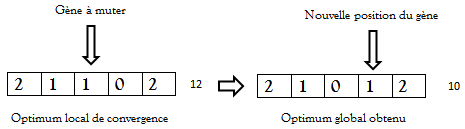
\includegraphics[scale=.6]{images/local_search_fig.png}
			\caption{Application de l'algorithme de recherche de meilleure solution à un chromosome}
			\label{fig:local_search_fig}
		\end{center}
	\end{figure} 
	
	\subsubsection{Table de Hash}
	Dans le processus de résolution des problèmes à l'aide des algorithmes génétiques, au fur et à mesure que les générations passent, la population évolue et la diversité au sein de cette dernière diminue amenant les mêmes chromosomes à être régulièrement réévalués. Dans les faits, l'effort de calculs dépensé à évaluer le "\emph{fitness}" dépasse celui dépensé sur les opérateurs génétiques. En utilisant une table de hash afin de stocker les chromosomes récemment évalués, une amélioration significative des performances peut être constatée. Nous avons donc utilisé un dictionnaire ou tableau associatif afin de stocker ces derniers. \\
	\\
	\begin{algorithm}[H]
 		\caption{Algorithme implémentant l'utilisation de la table de hash dans nos méthodes proposées}
 		\label{alg:table_hash}
 		\KwData{chromosome, table\_hash, max\_len}
 		%\KwResult{eval}
 		\BlankLine
 		
 		solution $\gets$ chromosome.solution\;
 		\eIf {solution in table\_hash}
 		{
 			indice $\gets$ table\_hash[solution] \;
 			chromosome.valeurFitness $\gets$ table\_hash[solution][valeurFitness] \;
 		}
 		{
			chromosome.valeurFitness  $\gets$ evaluation(solution) \;
			table\_hash.ajouter([solution, chromosome.valeurFitness])\;	
			\If{longueur(table\_hash) > max\_len}
			{
				table\_hash.enleverDernier() \;
			}
 		}
 	
	\end{algorithm}
	
	\section*{Conclusion}
	\addcontentsline{toc}{section}{Conclusion}
	Cette deuxième partie a présenté le modèle utilisé dans la résolution du PSP ainsi que les aspects communs aux deux solutions proposées. Dans un second temps, nous avons présenté et détaillé deux approches heuristiques basées sur les algorithmes génétiques parallèles utilisées afin de résoudre le problème. Dans la suite, nous présentons nos deux approches et analysons les résultats afin de les comparer à l'état de l'art en la matière.
